\chapter{Implementation} % (fold)
\label{chap:Implementation}
% python protocol "Next Header:8,Hdr Ext Len:8,Routing Type:8,Num. Dst:8,Flags:2,Hops:6,Reserved:24,Delivery Map:32,Router Map:32,Address List:128"
% python protocol "Next Header:8,Hdr Ext Len:8,Routing Type:8,Segments Left:8,Num. Dst:8,Flags:2,Hops:6,Reserved:16,Delivery Map:32,Router Map:32,Address List:128"

\begin{figure}[h!]
\centering
\begin{lstlisting}[xleftmargin=.07\textwidth]
 0                   1                   2                   3
 0 1 2 3 4 5 6 7 8 9 0 1 2 3 4 5 6 7 8 9 0 1 2 3 4 5 6 7 8 9 0 1
+-+-+-+-+-+-+-+-+-+-+-+-+-+-+-+-+-+-+-+-+-+-+-+-+-+-+-+-+-+-+-+-+
|  Next Header  |  Hdr Ext Len  |  Routing Type |    Num. Dst   |
+-+-+-+-+-+-+-+-+-+-+-+-+-+-+-+-+-+-+-+-+-+-+-+-+-+-+-+-+-+-+-+-+
|Fl.|    Hops   |                    Reserved                   |
+-+-+-+-+-+-+-+-+-+-+-+-+-+-+-+-+-+-+-+-+-+-+-+-+-+-+-+-+-+-+-+-+
|                          Delivery Map                         |
+-+-+-+-+-+-+-+-+-+-+-+-+-+-+-+-+-+-+-+-+-+-+-+-+-+-+-+-+-+-+-+-+
|                           Router Map                          |
+-+-+-+-+-+-+-+-+-+-+-+-+-+-+-+-+-+-+-+-+-+-+-+-+-+-+-+-+-+-+-+-+
|                                                               |
.                                                               .
.                          Address List                         .
.                                                               .
|                                                               |
+-+-+-+-+-+-+-+-+-+-+-+-+-+-+-+-+-+-+-+-+-+-+-+-+-+-+-+-+-+-+-+-+
\end{lstlisting}
\caption{Python: MEADcast Header}
\end{figure}

\begin{figure}[h!]
\centering
\begin{lstlisting}[xleftmargin=.07\textwidth]
 0                   1                   2                   3
 0 1 2 3 4 5 6 7 8 9 0 1 2 3 4 5 6 7 8 9 0 1 2 3 4 5 6 7 8 9 0 1
+-+-+-+-+-+-+-+-+-+-+-+-+-+-+-+-+-+-+-+-+-+-+-+-+-+-+-+-+-+-+-+-+
|  Next Header  |  Hdr Ext Len  |  Routing Type | Segments Left |
+-+-+-+-+-+-+-+-+-+-+-+-+-+-+-+-+-+-+-+-+-+-+-+-+-+-+-+-+-+-+-+-+
|    Num. Dst   |Fl.|    Hops   |            Reserved           |
+-+-+-+-+-+-+-+-+-+-+-+-+-+-+-+-+-+-+-+-+-+-+-+-+-+-+-+-+-+-+-+-+
|                          Delivery Map                         |
+-+-+-+-+-+-+-+-+-+-+-+-+-+-+-+-+-+-+-+-+-+-+-+-+-+-+-+-+-+-+-+-+
|                           Router Map                          |
+-+-+-+-+-+-+-+-+-+-+-+-+-+-+-+-+-+-+-+-+-+-+-+-+-+-+-+-+-+-+-+-+
|                                                               |
.                                                               .
.                          Address List                         .
.                                                               .
|                                                               |
+-+-+-+-+-+-+-+-+-+-+-+-+-+-+-+-+-+-+-+-+-+-+-+-+-+-+-+-+-+-+-+-+

\end{lstlisting}
\caption{Current: MEADcast Header}
\end{figure}

% \paragraph{Routing Type} % (fold)
% \label{par:Routing Type}
% Since there is no existing Routing Type for MEADcast we use the experimental
%     values of 253 and 254 according to RFC3692 \cite{rfc3692_ipv6_rt_type}.
% % paragraph Routing Type (end)
%
% \paragraph{Segments Left} % (fold)
% \label{par:Segments Left}
% Fixed to zero and is not altered by MEADcast routers.
% Thereby intermediate nodes, which does not recognize the used Routing type
%     value must ignore the MEADcast header and process the next header
%     \cite{rfc8200_ipv6_hdr}.
% % paragraph Segments Left (end)
%
% \paragraph{Number of Destinations} % (fold)
% \label{par:Number of Destinations}
% Indicates the length of the address list.
% % paragraph Number of Destinations (end)
%
% \paragraph{Flags} % (fold)
% \label{par:Flags}
% 1 bit discovery and 1 bit response.
% % paragraph Flags (end)
%
% \paragraph{Hops} % (fold)
% \label{par:Hops}
% This field is used during the discovery phase.
% The sender initializes the field with zero and gets incremented by each
%     MEADcast router.
% % paragraph Hops (end)
%
% \paragraph{Delivery Map} % (fold)
% \label{par:Delivery Map}
% Bitmap indicating, whether an address in the address list needs to be
%     delivered.
% % paragraph Delivery Map (end)
%
% \paragraph{Router Map} % (fold)
% \label{par:Router Map}
% Immutable bitmap indicating, whether an address in the address list is a router.
% % paragraph Router Map (end)
%
% \paragraph{Address List} % (fold)
% \label{par:Address List}
% List of length ``\texttt{Number of Destinations}'' containing IPv6 addresses.
% % paragraph Address List (end)

\bgroup
\begin{table}[h!]
\centering
\def\arraystretch{1.5}%  1 is the default
\setlength{\tabcolsep}{1.2em}
\begin{tabularx}{\textwidth}{lX}
% \toprule
% \textbf{Field}& \textbf{Desciption} \\
% \midrule
Routing Type  & Since there is no existing Routing Type for MEADcast we use the
                experimental values of 253 and 254 according to RFC3692
                \cite{rfc3692_ipv6_rt_type}.\\
Segments Left & Fixed to zero and is not altered by MEADcast routers. Thereby
                intermediate nodes, which does not recognize the used Routing
                type value must ignore the MEADcast header and process the next
                header \cite{rfc8200_ipv6_hdr}.\\
Num. Dst.     & Indicates the length of the address list. \\
Flags         & 1 bit discovery, 1 bit response        \\
Hops          & This field is used during the discovery phase. The sender
                initializes the field with zero and gets incremented by each
                MEADcast router. \\
Delivery Map  & Bitmap indicating, whether an address in the address list needs
                to be delivered.\\
Router Map    & Bitmap indicating, whether an address in the address list is a
                router.\\
Address List  & Variable length list of IPv6 addresses. \\
% \bottomrule
\end{tabularx}
\caption{MEADcast Header field description}
\label{tab:my-table}
\end{table}
\egroup

\section{Router} % (fold)
\label{sec:Router}
This section provides an overview of the MEADcast router implementation in the
    Linux Kernel.
The MEADcast routing software is developed and tested using the latest stable
    Kernel release, version 6.5.3, at the time of development.
MEADcast routing capabilities are tightly coupled to the flow of IPv6 packets
    through the Kernel network stack, making it infeasible to create a separate
    Kernel module loadable at runtime.
Therefore, we decided to extend the IPv6 module with MEADcast capability.
This feature can be enabled or disabled at compile-time using the
    \inlinelst{CONFIG\_IPV6\_MEADCAST} flag.
To avoid the burden of recompiling or switching the kernel to enable or disable
    MEADcast support, we introduce a runtime configuration flag.
This flag is managed through Sysctl, providing the virtual file
    \inlinelst{/proc/sys/net/ipv6/meadcast/enable}, which contains either 0 for
    disabled and 1 for enabled.
For instance, the root user can enable MEADcast support by running the command
    \inlinelst{"echo 1 > /proc/sys/net/ipv6/meadcast/enable"}.
However, it is crucial to ensure that this additional check does not adversely
    impact performance compared to a plain kernel, as it could potentially
    affect the reliability of experimental results.

As illustrated in \autoref{sub:Network Stack}, packets not designated to the
    router itself follow the ``forwarding'' packet flow in the Kernel.
IPv6 extension headers of these packets are normally ignored by the Kernel
    (except for the Router Alert extension).
Consequently, we embedded the entry point for MEADcast processing at the end of
    the \inlinelst{ip6\_forward} method located in
    \inlinelst{net/ipv6/ipv6\_output.c}.
If a packet contains the routing header extension the \inlinelst{mdc\_rcv}
    method located in \inlinelst{net/ipv6/mdcast.c} gets invoked.
This method performs basic sanity checks on the MEADcast header and then
    invokes \inlinelst{mdc\_dcv\_rcv} for discovery and
    \inlinelst{mdc\_data\_rcv} for data packets.

% discovery
% - validation
% - increment hop counter
% - clone socket buffer of incomming packet (discovery response)
% - update dst and src ip of discovery response
\textit{Discovery}: First, discovery packets get validated and the hop counter
    in the MEADcast header is incremented.
To create a discovery response the socket buffer struct of the incoming
    discovery request is cloned.
By this, we solely have to update the IP source and destination field of the
    cloned packet, set the response flag, and perform a routing table lookup
    for the sender's address.
The source IP address of the discovery response is set to the IP address
    associated with the interface returned from the routing lookup.
Lastly, the \inlinelst{dst\_output} method is invoked, dispatching the packet to
    the corresponding layer 2 handler.
The processing of the original packet does not need further handling, as it is
    already correctly done by the default forwarding flow.

\textit{Data}: Data packets undergo several steps upon arrival at the MEADcast
    router.
Firstly, they are validated, and the hop counter in the MEADcast header is
    incremented.
Subsequently, the router iterates over the Delivery and Router Bitmap to
    identify undelivered routers (indices set in both bitmaps).
During this iteration, if the router is not the last undelivered router in the
    sequence, the socket buffer of the original packet is cloned and forwarded
    accordingly.
However, if the router is the last undelivered router, the original packet can
    be forwarded without the need for costly replication.
To determine whether to clone the packet, the routers monitors whether an 
    undelivered router at index $r1$ has a successor (another undelivered
    router) at index $r2$, with $r1 < r2$.
The algorithm's specifics are depicted in \autoref{fig:router_hdr_parsing}.

For each undelivered router $R_u$ in the MEADcast header the processing router
    $R_p$ decides whether to deliver the data via MEADcast or IP unicast.
If the IP address of $R_u$ in the MEADcast header is owned by the processing
    router $R_p$, all designated endpoints will be delivered via IP unicast.
If the number of endpoints of the considered router $R_u$ from the MEADcast
    header is below a certain threshold, the processing router $R_p$ performs a
    premature MEADcast to IP unicast transformation.
For example, if $R_u$ has one designated endpoint $R_p$ could perform a
    premature MEADcast to IP unicast transformation which possibly may
    improve the performance.

% Search for first router
%
% - validation
% - increment hop count
% - iterate bitmaps
%   - check which routers aren't delivered yet
%   - if router is not last undelivered router create a copy of socket buffer struct
%   - else use incoming one
% - forwarding
%   - if router addr in bitmap is of router or less than min_dsts eps -> m2u
%   - else: update bitmap (set all others to delivered), update ip dst field
% - m2u
%   - copy IP hdr in front of l3 header
%   - update skb pointers
%   - recalc checksum
\begin{figure}
    \begin{center}
        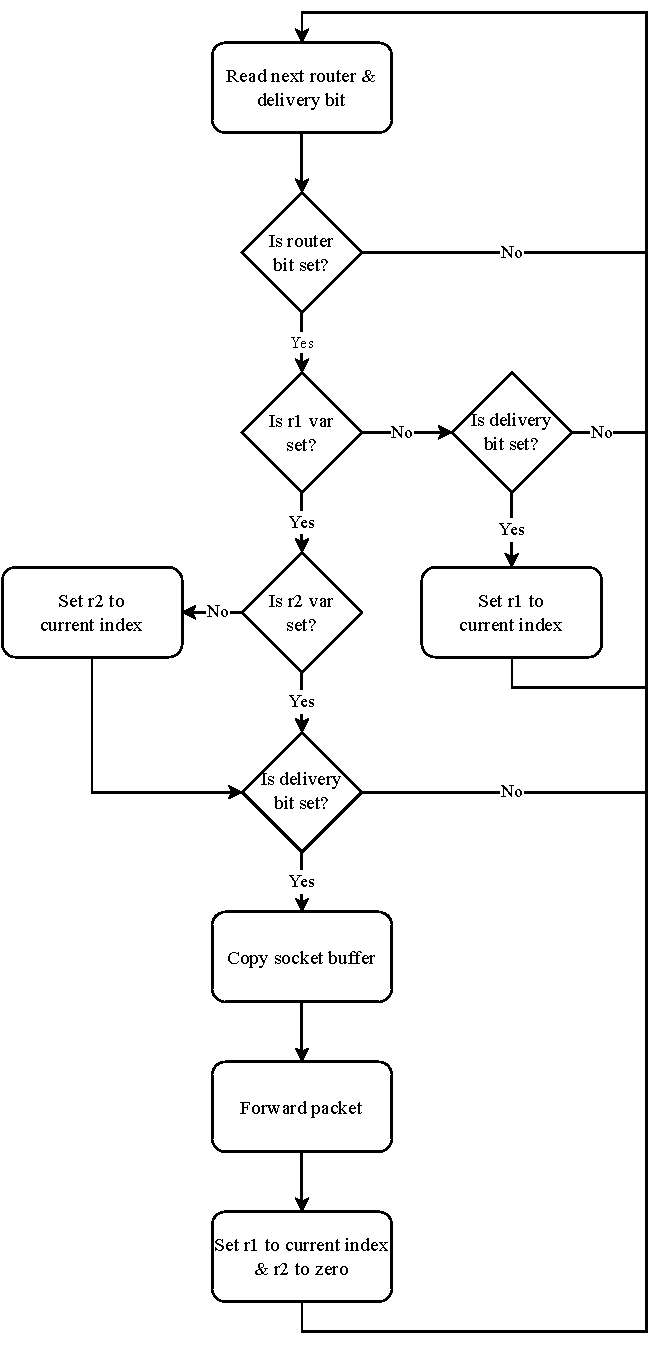
\includegraphics[scale=1]{router_hdr_parsing.pdf}
    \end{center}
    \caption{Router header parsing}
    \label{fig:router_hdr_parsing}
\end{figure}

\begin{figure}
    \begin{center}
        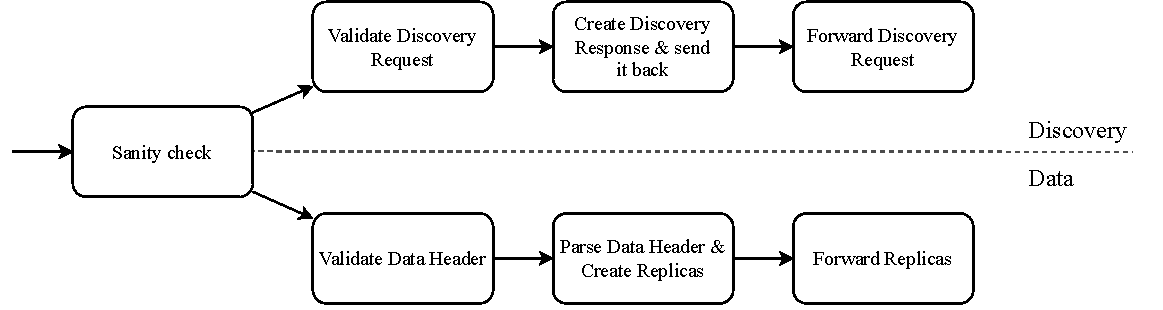
\includegraphics[width=\textwidth]{router_procedure.pdf}
    \end{center}
    \caption{MEADcast router procedure}
    \label{fig:router_procedure}
\end{figure}
% section Router (end)


\section{Sender} % (fold)
\label{sec:Sender}
% - TUN
% - Judy Array to quickly find IPs
% - Tree for grouping
% - grouping algorithm
% section Sender (end)


\section{Testbed} % (fold)
\label{sec:Testbed_Implementation}
% - python script reading json
% - kvm, direct kernel boot, debian nocloud image
% - chrony time sync (had to change boot param on host system)
% section Testbed (end)


% chapter Implementation (end)
